Dentro de este capítulo de muestran las aplicaciones que se ejecutan dentro de servidores Web, se seleccionaron dos servidores, Tornado y NodeJs. Un pequeño resumen de cada uno podrá ser encontrado en sus respectivas secciones.

%--------------------------------------------------
\section{Node.JS con Express}
Node.js ® es una construcción en tiempo de ejecución JavaScript creado en el motor de JavaScript V8 de Chrome. Node.js utiliza un modelo de E/S no bloquantes y controlado por eventos que lo hace liviano y eficiente. El ecosistema de paquetes de Node.js, npm, es el mayor ecosistema de bibliotecas de código abierto del mundo \cite{Node}. El logotipo de Node.js se encuentra en la figura \ref{node}

\FloatBarrier
\begin{figure}[htbp!]
		\centering
			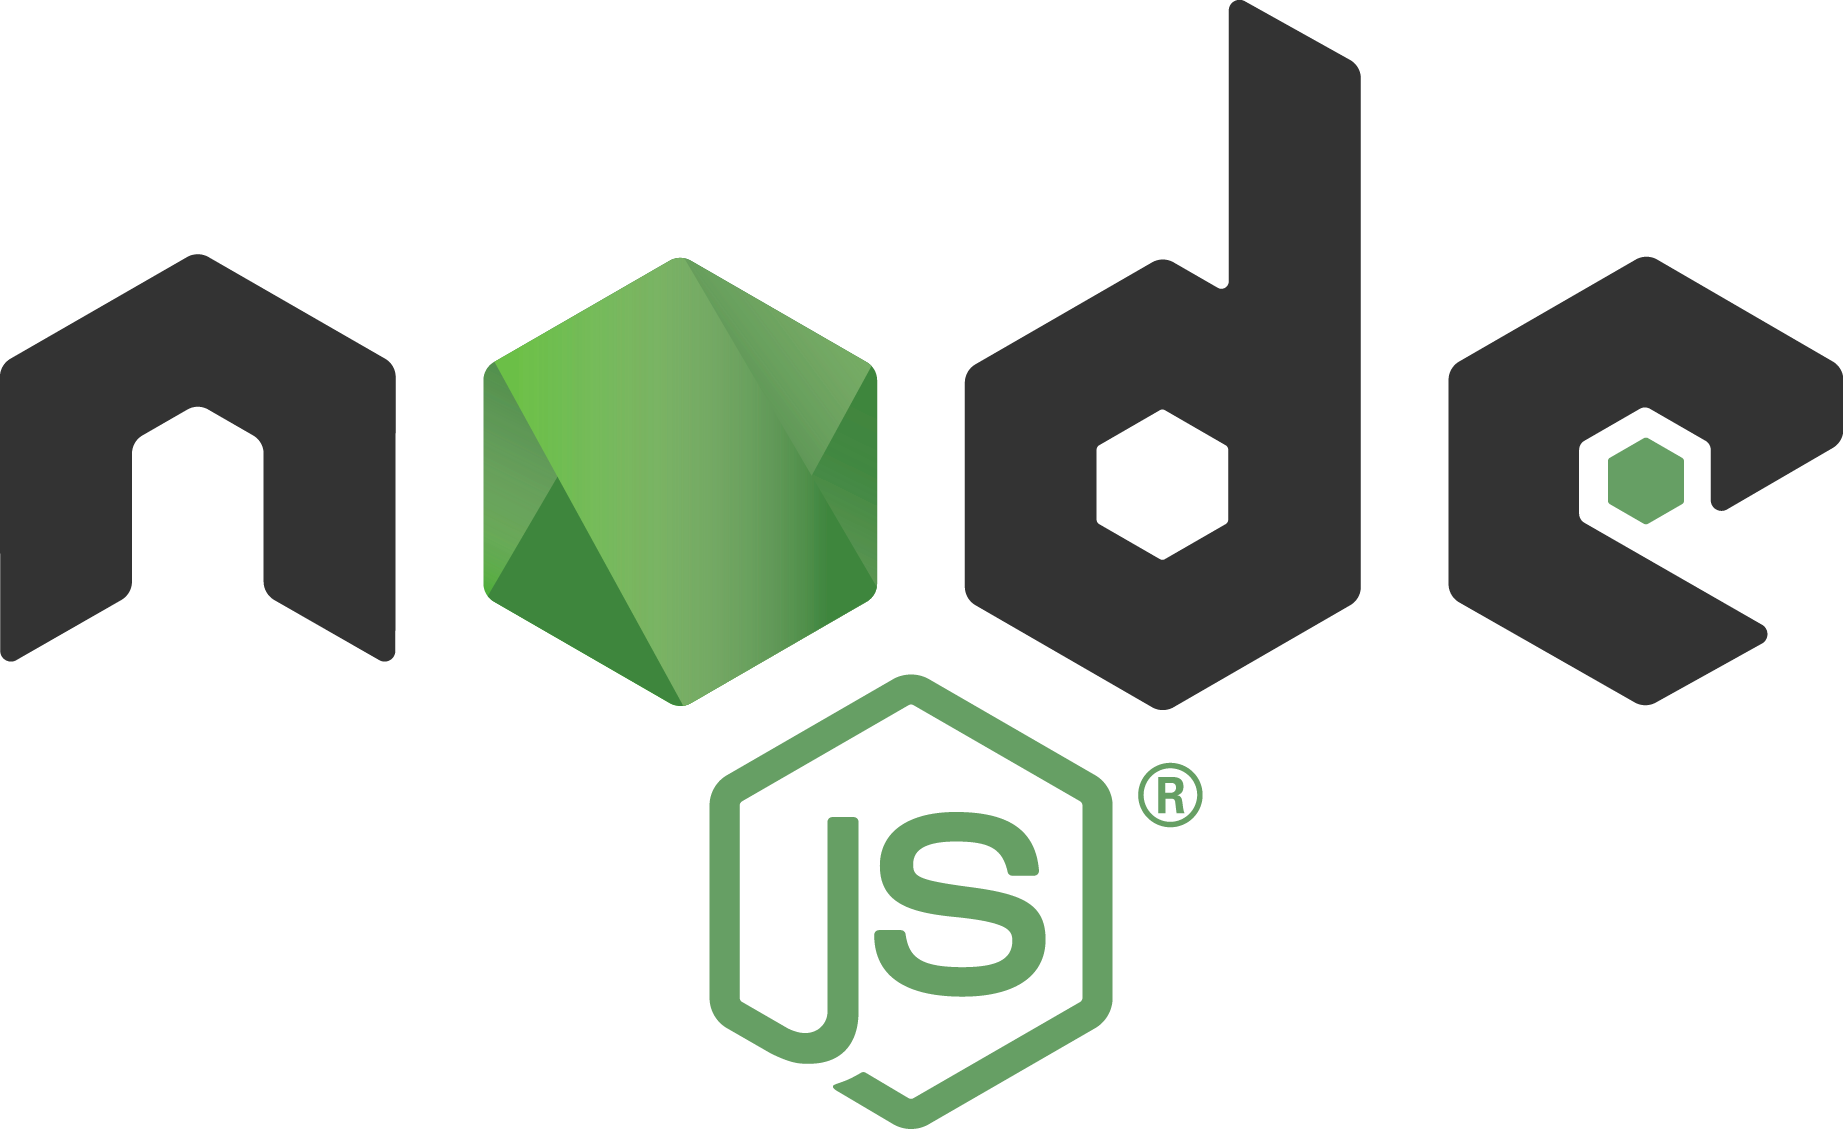
\includegraphics[width=0.3 \textwidth]{imagenes/logoNode}
		\caption{Logo de Node.js. \cite{Node}.}
		\label{node}
\end{figure}
\FloatBarrier

Express.js, o simplemente Express, es un framework Web para Node.js, lanzado como software libre y de código abierto bajo la Licencia MIT. Está diseñado para crear aplicaciones Web y API. Express ha sido llamado como framework base estándar para Node.js \cite{Express}. El respectivo logotipo del framework se puede visualizar en la figura \ref{Express}


\FloatBarrier
\begin{figure}[htbp!]
		\centering
			
\includegraphics[width=0.3 \textwidth]{imagenes/Expressjs}
		\caption{Logo de Express. \cite{Express}.}
		\label{Express}
\end{figure}
\FloatBarrier
\subsection{Panel de Administración (PA)}
A continuación en la figura \ref{image:arquitecturaPA} se presenta la arquitectura del prototipo Panel de Administración.
\FloatBarrier
\begin{figure}[htbp!]
		\centering
			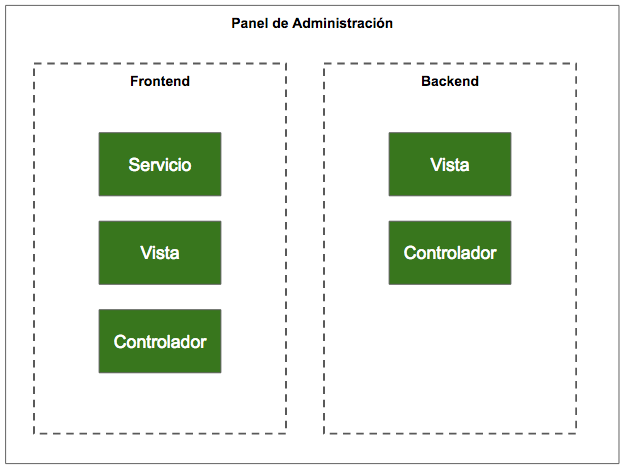
\includegraphics[width=.9 \textwidth]{imagenes/Arquitecturas/arquiRuben}
		\caption{Arquitectura del módulo PA. }
		\label{image:arquitecturaPA}
\end{figure}
\FloatBarrier
La descripción de cada elemento de la arquitectura es la siguiente:
\begin{itemize}
\item Frontend: Se enfoca en el usuario, en todo con lo que podemos interactuar y lo que vemos mientras navegamos.
\begin{itemize}
\item Servicio: Se encarga de hacer peticiones HTTP a un servicio externo (API REST, microservicio, Web service)
\item Vista: Se refiere a la pantalla que le es mostrada al usuario final.
\item Controlador: Se encarga de toda la lógica de negocio de la vista.
\end{itemize}
\item Backend: Está enfocado en hacer que todo lo que está detrás de un sitio web funcione correctamente.
\begin{itemize}
\item Vista: Se refiere a la pantalla que le es mostrada al usuario final.
\item Controlador: Controlador: Se encarga de toda la lógica de negocio de la vista.
\end{itemize}
\end{itemize}


%--------------------------------------------------
\subsection{Prototipo 1: Diseño inicial del Panel de Administración}

%--------------------------------------------------
\subsubsection{Análisis}


%--------------------------------------------------
\subsubsection{Diseño}

\title{\textbf{Diseño de interfaz de usuario \\}}
La Figura \ref{image:disenogeneralPA} muestra el diseño de la interfaz de usuario que contendrá el Panel de Administración.
\FloatBarrier
\begin{figure}[htbp!]
		\centering
			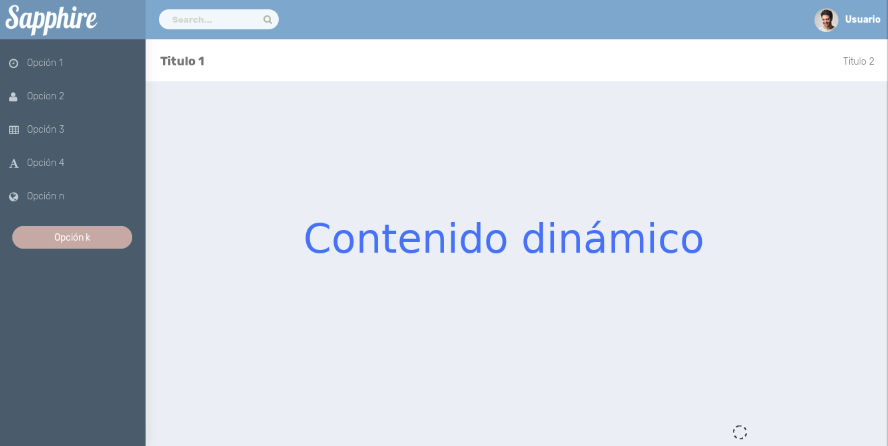
\includegraphics[width=.8 \textwidth]{imagenes/UI/middlewareP1}
		\caption{Diseño general del PA.}
		\label{image:disenogeneralPA}
\end{figure}
\FloatBarrier

La Figura \ref{PA:1} muestra como se ve la interfaz de usuario del Panel de Administración desde una computadora.
\FloatBarrier
\begin{figure}[htbp!]
		\centering
			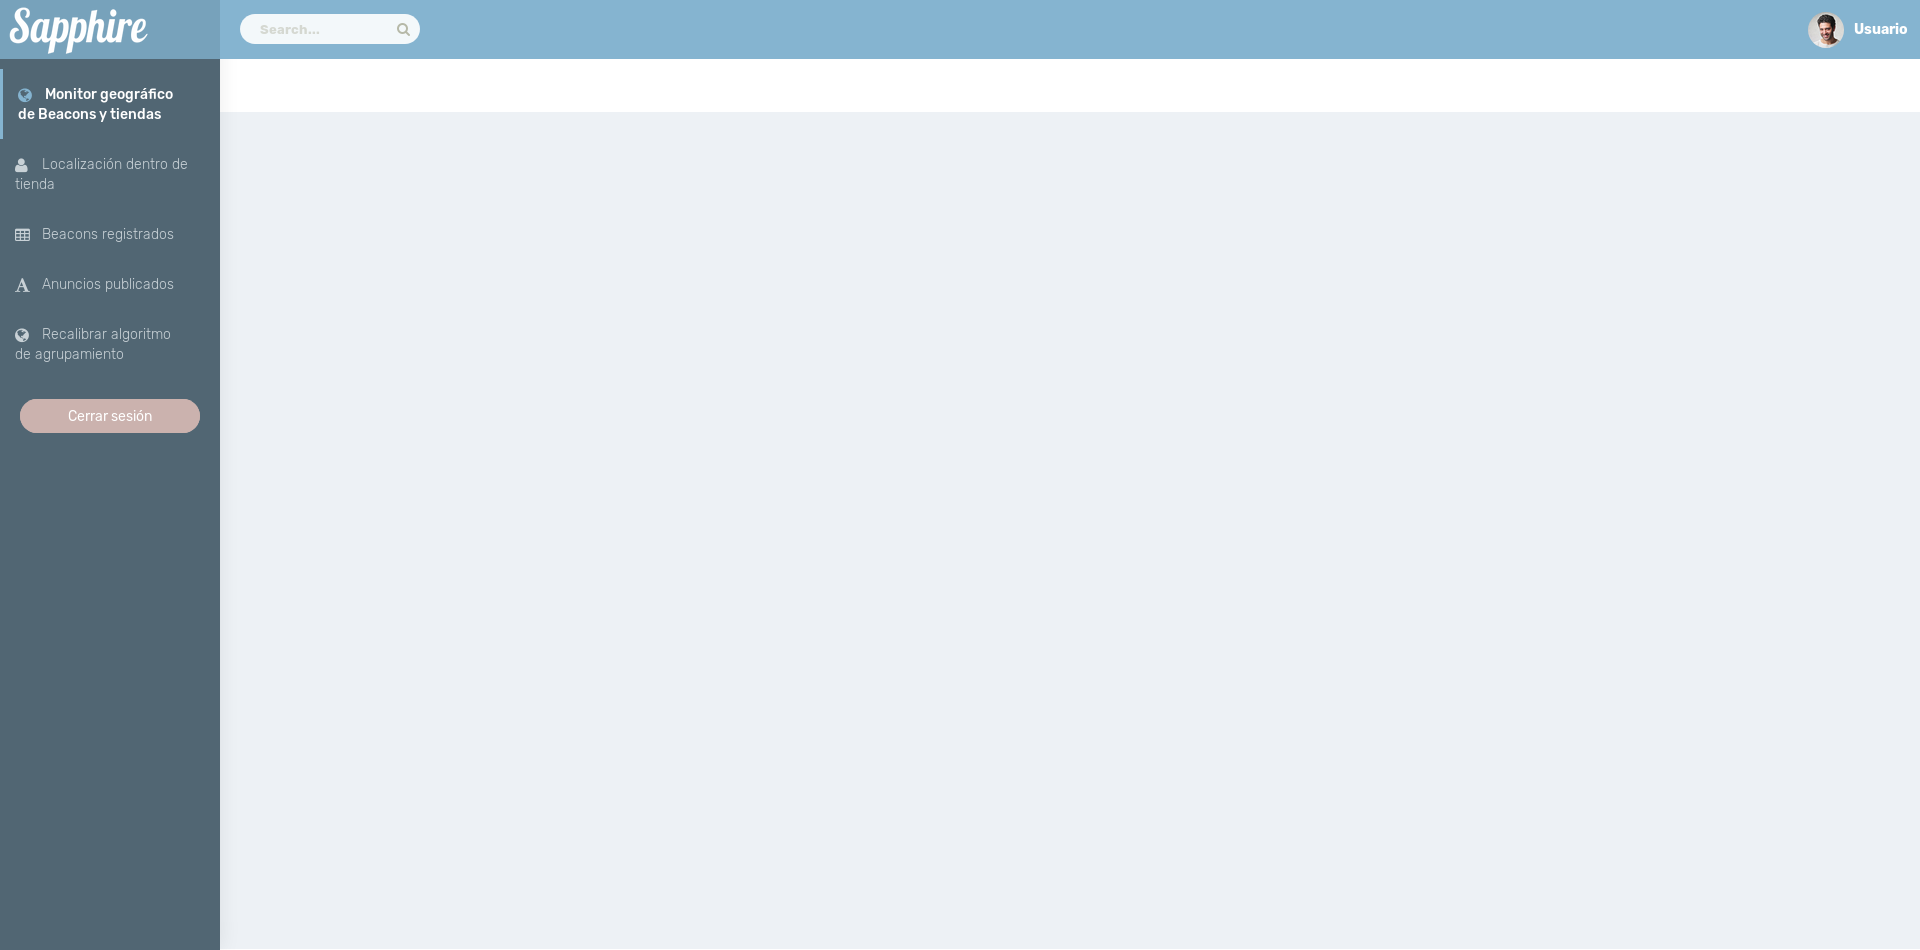
\includegraphics[width=.9 \textwidth]{imagenes/panelAdmin/panelAdmin}
		\caption{UIPanel1: Diseño computadora.}
		\label{PA:1}
\end{figure}
\FloatBarrier
La Figura \ref{PA:2} muestra como se ve la interfaz de usuario del Panel de Administración desde una tableta.
\FloatBarrier
\begin{figure}[htbp!]
		\centering
			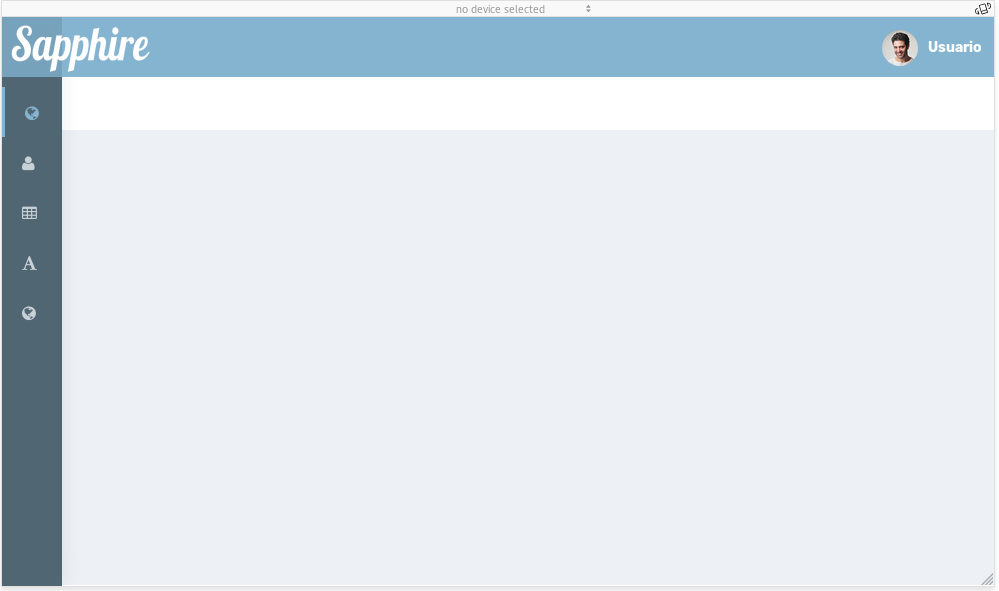
\includegraphics[width=.9 \textwidth]{imagenes/panelAdmin/tab}
		\caption{UIPanel2: Diseño tableta.}
		\label{PA:2}
\end{figure}
\FloatBarrier
